\documentclass[10pt]{beamer}\usepackage[]{graphicx}\usepackage[]{color}
% maxwidth is the original width if it is less than linewidth
% otherwise use linewidth (to make sure the graphics do not exceed the margin)
\makeatletter
\def\maxwidth{ %
  \ifdim\Gin@nat@width>\linewidth
    \linewidth
  \else
    \Gin@nat@width
  \fi
}
\makeatother

\definecolor{fgcolor}{rgb}{0.345, 0.345, 0.345}
\newcommand{\hlnum}[1]{\textcolor[rgb]{0.686,0.059,0.569}{#1}}%
\newcommand{\hlstr}[1]{\textcolor[rgb]{0.192,0.494,0.8}{#1}}%
\newcommand{\hlcom}[1]{\textcolor[rgb]{0.678,0.584,0.686}{\textit{#1}}}%
\newcommand{\hlopt}[1]{\textcolor[rgb]{0,0,0}{#1}}%
\newcommand{\hlstd}[1]{\textcolor[rgb]{0.345,0.345,0.345}{#1}}%
\newcommand{\hlkwa}[1]{\textcolor[rgb]{0.161,0.373,0.58}{\textbf{#1}}}%
\newcommand{\hlkwb}[1]{\textcolor[rgb]{0.69,0.353,0.396}{#1}}%
\newcommand{\hlkwc}[1]{\textcolor[rgb]{0.333,0.667,0.333}{#1}}%
\newcommand{\hlkwd}[1]{\textcolor[rgb]{0.737,0.353,0.396}{\textbf{#1}}}%
\let\hlipl\hlkwb

\usepackage{framed}
\makeatletter
\newenvironment{kframe}{%
 \def\at@end@of@kframe{}%
 \ifinner\ifhmode%
  \def\at@end@of@kframe{\end{minipage}}%
  \begin{minipage}{\columnwidth}%
 \fi\fi%
 \def\FrameCommand##1{\hskip\@totalleftmargin \hskip-\fboxsep
 \colorbox{shadecolor}{##1}\hskip-\fboxsep
     % There is no \\@totalrightmargin, so:
     \hskip-\linewidth \hskip-\@totalleftmargin \hskip\columnwidth}%
 \MakeFramed {\advance\hsize-\width
   \@totalleftmargin\z@ \linewidth\hsize
   \@setminipage}}%
 {\par\unskip\endMakeFramed%
 \at@end@of@kframe}
\makeatother

\definecolor{shadecolor}{rgb}{.97, .97, .97}
\definecolor{messagecolor}{rgb}{0, 0, 0}
\definecolor{warningcolor}{rgb}{1, 0, 1}
\definecolor{errorcolor}{rgb}{1, 0, 0}
\newenvironment{knitrout}{}{} % an empty environment to be redefined in TeX

\usepackage{alltt}


%\input{slides_header.tex}
\usepackage{graphicx}
\usepackage{hyperref, url}
\hypersetup{colorlinks,citecolor=myorange,filecolor=red,linkcolor=brown,urlcolor=blue}

\usepackage{longtable,booktabs}
\usepackage{amssymb,amsmath}
\usepackage{animate}
\usepackage{subfig}
\usepackage{tikz}
\usetikzlibrary{shapes.geometric, arrows,shapes.symbols,decorations.pathreplacing}
\tikzstyle{startstop} = [rectangle, rounded corners, minimum width=3cm, minimum height=1cm, draw=black, fill=pinkish,text width=3.5cm]
\tikzstyle{startstop2} = [rectangle, rounded corners, minimum width=3cm, minimum height=1cm, draw=black, fill=background,text width=4.5cm]
\tikzstyle{startstop3} = [rectangle, rounded corners, minimum width=3cm, minimum height=1cm, draw=black, fill=beige,text width=3.0cm]
\tikzstyle{startstop4} = [rectangle, rounded corners, minimum width=3cm, minimum height=1cm, draw=black, fill=pinkish,text width=4.5cm]
\tikzstyle{io} = [trapezium, trapezium left angle=70, trapezium right angle=110, minimum width=2cm, minimum height=1cm, text centered, draw=black, fill=blue!30,text width=1.5cm]
\tikzstyle{process} = [rectangle, minimum width=1cm, minimum height=1cm, text centered, draw=black, fill=orange!30,text width=2cm]
\tikzstyle{decision} = [diamond, minimum width=2cm, minimum height=1cm, text centered, draw=black, fill=green!30]
\tikzstyle{arrow} = [thick,->,>=stealth]
\tikzstyle{both} = [thick,<->,>=stealth, red]


% used for tree of stats tests in 001-introduction
\tikzstyle{startstopstats} = [rectangle, rounded corners, minimum width=2cm, minimum height=.5cm,text centered, draw=black, fill=red!30]
\tikzstyle{iostats} = [trapezium, trapezium left angle=70, trapezium right angle=110, minimum width=2cm, minimum height=.5cm, text centered, draw=black, fill=blue!30]
\tikzstyle{processstats} = [rectangle, minimum width=1.5cm, minimum height=.5cm, text centered, draw=black, fill=orange!30]
\tikzstyle{processbigstats} = [rectangle, minimum width=1.5cm, minimum height=.5cm, text centered, draw=black, fill=orange!30,text width=1.6cm]
\tikzstyle{decisionstats} = [rectangle, minimum width=1cm, minimum height=1cm, text centered, draw=black, fill=green!30,text width=1.6cm]
\tikzstyle{decisionbigstats} = [rectangle, minimum width=1cm, minimum height=1cm, text centered, draw=black, fill=yellow!30,text width=2cm]

\usepackage{pifont}% http://ctan.org/pkg/pifont
\newcommand{\cmark}{\ding{51}}%
\newcommand{\xmark}{\ding{55}}%

\usepackage{ulem} % for strikeout

\usepackage{xcolor}
\usepackage{color, colortbl}
\definecolor{lightgray}{RGB}{200,200,200}
\definecolor{palegray}{RGB}{221,221,221}
\definecolor{myblue}{RGB}{0,89,179}
\definecolor{myorange}{rgb}{0.776,0.357,0.157}
\definecolor{gray}{RGB}{110,110,110}
\definecolor{darkgray}{RGB}{100,100,100}
\definecolor{lightgray}{RGB}{200,200,200}
\definecolor{palegray}{RGB}{221,221,221}
\definecolor{turquoise}{RGB}{81,193,188}
\definecolor{tomato}{RGB}{255,136,136}
\definecolor{mandarina}{RGB}{229,169,25}
\definecolor{foreground}{RGB}{81,141,193}
\definecolor{background}{RGB}{246,244,240}
\definecolor{highlight}{RGB}{229,169,25}
\definecolor{lowlight}{RGB}{200,200,200}
\definecolor{beige}{RGB}{255,255,240}
\definecolor{pinkish}{RGB}{255,223,247}
\definecolor{darktangerine}{rgb}{1.0, 0.66, 0.07}
\definecolor{deepink}{RGB}{255,20,147}
%\usepackage{shadethm}
%\colorlet{shadecolor}{blue!15}
%\colorlet{shadecolor}{palegray}
%\setlength{\shadeboxrule}{.4pt}

%\newshadetheorem{thm}{Theorem}
%\newshadetheorem{defm}{Definition}
%\newshadetheorem{exm}{Exercise}
%\newshadetheorem{remarkm}{Remark}
%\definecolor{shadethmcolor}{HTML}{EDF8FF}
%\definecolor{shadethmcolor}{RGB}{221,221,221}
%\definecolor{shaderulecolor}{HTML}{45CFFF}
%\definecolor{shaderulecolor}{RGB}{0,89,179}
%\setlength{\shadeboxrule}{.4pt}



\usepackage{epsfig}

\newcommand{\code}[1]{\texttt{#1}}
\newcommand{\blue}[1]{\textcolor{blue}{#1}}
\newcommand{\red}[1]{\textcolor{red}{#1}}

\usepackage{comment}

\makeatletter

\def \iqsssectiontitleheader {}

\newcommand{\iqsssectiontitle}[1]{
	\def \iqsssectiontitleheader{#1}
}

\@ifundefined{insertmainframenumber}
{%
	% \insertmainframenumber not defined
	\newcommand{\insertmainframenumber}{\inserttotalframenumber}
}
{%
	% \insertmainframenumber already defined
}%


\AtBeginSection[]{
	\title{\insertsectionhead}
	{
		%\definecolor{white}{RGB}{140,193,250}
		%\definecolor{white}{RGB}{200,200,200}
		%\definecolor{white}{RGB}{242,244,247}
		\definecolor{white}{RGB}{0,89,179}
		%\definecolor{iqss@orange}{rgb}{1,1,1}
		\ifnum \insertmainframenumber > \insertframenumber
		%\setbeamercolor{background canvas}{bg=myblue}
		%\setbeamercolor{normal text}{fg=black,bg=white}
		%\setbeamercolor{frametitle}{fg=red}
		%\setbeamercolor{section in toc}{fg=myblue, bg=white}
		%\setbeamercolor{subsection in toc}{fg=myblue, bg=white}
		\frame{
			\frametitle{\iqsssectiontitleheader}
			\tableofcontents[currentsection]
		}
		\else
		\frame{
			\frametitle{Backup Slides}
			\tableofcontents[sectionstyle=shaded/shaded,subsectionstyle=shaded/shaded/shaded]
		}
		\fi
	}
}
\makeatother
%\graphicspath{{/home/sahir/git_repositories/EPIB607/resources/assets/slides/figure/}}


\usepackage{fontspec}
%\setsansfont{Fira Sans}
%\setmonofont{Fira Mono}
%\setsansfont[ItalicFont={Fira Sans Light Italic},BoldFont={Fira Sans},BoldItalicFont={Fira Sans Italic}]{Fira Sans Light}
%\setmonofont[BoldFont={Fira Mono Medium}]{Fira Mono}

\def\installpath{/usr/local/share/texmf/fonts/opentype/libertinus/}
\setmainfont{LibertinusSerif}[
UprightFont    = *-Regular,
BoldFont       = *-Bold,
ItalicFont     = *-Italic,
BoldItalicFont = *-BoldItalic,
Ligatures      = TeX,
Extension      = .otf,
Path           = \installpath/
]

\setsansfont{LibertinusSerif}[
UprightFont    = *-Regular,
BoldFont       = *-Bold,
ItalicFont     = *-Italic,
BoldItalicFont = *-BoldItalic,
Ligatures      = TeX,
Extension      = .otf,
Path           = \installpath/
]


%\setmonofont{LibertinusSerif}[
%UprightFont    = *-Regular,
%BoldFont       = *-Bold,
%ItalicFont     = *-Italic,
%BoldItalicFont = *-BoldItalic,
%Ligatures      = TeX,
%Extension      = .otf,
%Path           = \installpath/
%]






\newcommand\Wider[2][3em]{%
	\makebox[\linewidth][c]{%
		\begin{minipage}{\dimexpr\textwidth+#1\relax}
			\raggedright#2
		\end{minipage}%
	}%
}


\newcommand {\framedgraphic}[1] {
	\begin{figure}
		\centering
		\includegraphics[width=\textwidth,height=0.9\textheight,keepaspectratio]{#1}
	\end{figure}
}


\newcommand {\framedgraphiccaption}[2] {
	\begin{figure}
		\centering
		\includegraphics[width=\textwidth,height=0.8\textheight,keepaspectratio]{#1}
		\caption{#2}
	\end{figure}
}




\setbeamercolor{itemize item}{fg=myblue}
\setbeamercolor{itemize subitem}{fg=myorange}
%\setbeamertemplate{itemize item}[square]
\setbeamertemplate{itemize item}[circle]
\setbeamertemplate{itemize subitem}[triangle]
\setbeamertemplate{blocks}[rounded][shadow=true]
\setbeamercolor{block body alerted}{bg=alerted text.fg!10}
\setbeamercolor{block title alerted}{bg=alerted text.fg!20}
\setbeamercolor{block body}{bg=structure!10}
\setbeamercolor{block title}{bg=structure!20}
\setbeamercolor{block body example}{bg=green!10}
\setbeamercolor{block title example}{bg=green!20}


\makeatletter
\newenvironment<>{proofs}[1][\proofname]{%
	\par
	\def\insertproofname{#1\@addpunct{.}}%
	\usebeamertemplate{proof begin}#2}
{\usebeamertemplate{proof end}}
\newenvironment<>{proofc}{%
	\setbeamertemplate{proof begin}{\begin{block}{}}
		\par
		\usebeamertemplate{proof begin}}
	{\usebeamertemplate{proof end}}
	\newenvironment<>{proofe}{%
		\par
		\pushQED{\qed}
		\setbeamertemplate{proof begin}{\begin{block}{}}
			\usebeamertemplate{proof begin}}
		{\popQED\usebeamertemplate{proof end}}
\makeatother


\makeatletter
\newenvironment<>{exams}[1][\proofname]{%
	\par
	\def\insertproofname{#1\@addpunct{.}}%
	\usebeamertemplate{example begin}#2}
{\usebeamertemplate{example end}}
\newenvironment<>{examc}{%
	\setbeamertemplate{exam begin}{\begin{block}{}}
		\par
		\usebeamertemplate{exam begin}}
	{\usebeamertemplate{exam end}}
	\newenvironment<>{exame}{%
		\par
		\pushQED{\qed}
		\setbeamertemplate{exam begin}{\begin{block}{}}
			\usebeamertemplate{exam begin}}
		{\popQED\usebeamertemplate{exam end}}
		\makeatother

%\definecolor{mycolor}{HTML}{F7F8E0}
%\declaretheorem[shaded={bgcolor=mandarina}]{theo}
%\declaretheorem[shaded={bgcolor=mycolor}]{propo}
%\declaretheorem[shaded={bgcolor=green!80!black!30}]{remark}

%\setbeamertemplate{navigation symbols}{\usebeamercolor[fg]{title in head/foot}\usebeamerfont{title in head/foot}\insertframenumber}


%\setbeamertemplate{footline}{}

\beamertemplatenavigationsymbolsempty % toggle off if you want navigation symbols at the bottom

\setbeamertemplate{footline}
{ \usebeamercolor[fg]{page number in head/foot}%
	\usebeamerfont{page number in head/foot}%
	\hspace{1em}\insertsectionhead%
	\hfill%
	\insertframenumber\,/\,\hyperlinkappendixstart{\insertmainframenumber}
	\ifnum \thepage = \insertframeendpage{\small .}\else{\phantom{\small .}}\fi
	\hspace{1em}
	\vskip2pt%
}

%\newtheorem{proposition}[theorem]{Proposition}
%\newtheorem{exercise}[theorem]{Exercise}
%\newtheorem{remark}[theorem]{Remark}


\usepackage{amsthm}
\usepackage{thmtools}

\setbeamertemplate{theorems}[ams style] 
%\setbeamertemplate{theorems}[numbered] 
%\setbeamertemplate{corollary}[numbered] 
\newtheorem{proposition}{Proposition}
\newtheorem{exercise}{Exercise}
\newtheorem{remark}{Remark}
\newtheorem{exam}{Example}
%\newtheorem{proof}{Proof}
%\newtheorem{corollaries}[theorem]{Corollary}
\newcommand*{\theorembreak}{\usebeamertemplate{theorem end}\framebreak\usebeamertemplate{theorem begin}}



\setlength{\emergencystretch}{3em} % prevent overfull lines
\providecommand{\tightlist}{%
	\setlength{\itemsep}{0pt}\setlength{\parskip}{0pt}}

\newcommand\AddButton{%
	\setbeamertemplate{background canvas}{%
		\begin{tikzpicture}[remember picture,overlay]
		\node[anchor=west] at ([yshift=5pt,xshift=0.1em]current page.south west)
		{\hyperlink{toc}{\beamergotobutton{back to TOC}}};
		\end{tikzpicture}%
	}%
}


\titlegraphic{\hfill
\includegraphics[height=1cm]{/home/sahir/git_repositories/EPIB607/slides/mcgill_logo.png}}




\graphicspath{{/home/sahir/git_repositories/EPIB607/resources/assets/slides/figure/}}

%\let\oldShaded\Shaded
%\let\endoldShaded\endShaded
%\renewenvironment{Shaded}{\footnotesize\oldShaded}{\endoldShaded}
\IfFileExists{upquote.sty}{\usepackage{upquote}}{}
\begin{document}
	
	
	
	%\title{Introduction to Regression Trees}
	%\author{Sahir Bhatnagar \inst{1}}
	%\author[shortname]{Sahir Rai Bhatnagar, PhD Candidate (Biostatistics) }
	%\institute[shortinst]{Department of Epidemiology, Biostatistics and Occupational Health}
	
	\title{002 - Motivating Examples}
	\author{EPIB 607 - FALL 2020}
	\institute{
		Sahir Rai Bhatnagar\\
		Department of Epidemiology, Biostatistics, and Occupational Health\\
		McGill University\\
		
		\vspace{0.1 in}
		
		\texttt{sahir.bhatnagar@mcgill.ca}\\
		%\texttt{\url{https://sahirbhatnagar.com/EPIB607/}}
	}
	
	\date{slides compiled on \today}
	
	\maketitle

\section{Case study 1: Safety and immunogenicity of the ChAdOx1 nCoV-19	vaccine against SARS-CoV-2}


\begin{frame}{Early phase COVID-19 vaccine trial\footnote{\tiny\url{https://www.thelancet.com/journals/lancet/article/PIIS0140-6736(20)31604-4/fulltext}}}
	\centering
	
\includegraphics[scale=0.25]{002-cs1.png}	
\end{frame}




\begin{frame}{Phase 1/2 trial}
	\begin{itemize}
		\item The focus in phase 1/2 trials is looking at what the vaccine does to the body and what the body does with the vaccine in \textit{healthy} individuals
		\item Adults with no history of laboratory confirmed SARS-CoV-2 infection or of COVID-19-like symptoms were randomly assigned (1:1) to receive \textbf{ChAdOx1 nCoV-19} or \textbf{MenACWY} (Meningococcal) as a single intramuscular injection
		\item Convalescent plasma samples from adults with PCR-positive SARS-CoV-2 infection were obtained from symptomatic patients admitted to the hospitals to characterize the
		immunological properties of COVID-19\footnote{\tiny{Convalescent plasma is collected from someone who has recovered from a virus. When a person is infected with a virus, their body starts making antibodies to fight it. It is believed these antibodies could be the key ingredient for a treatment to help others with the same virus.}}
		\item The enzyme-linked immunosorbent assay (ELISA) technique was used to detect antibodies (i.e. levels of immunity)
		
	\end{itemize}
\end{frame}



\begin{frame}[fragile,plain]
	
	
\begin{knitrout}\tiny
\definecolor{shadecolor}{rgb}{0.969, 0.969, 0.969}\color{fgcolor}

{\centering 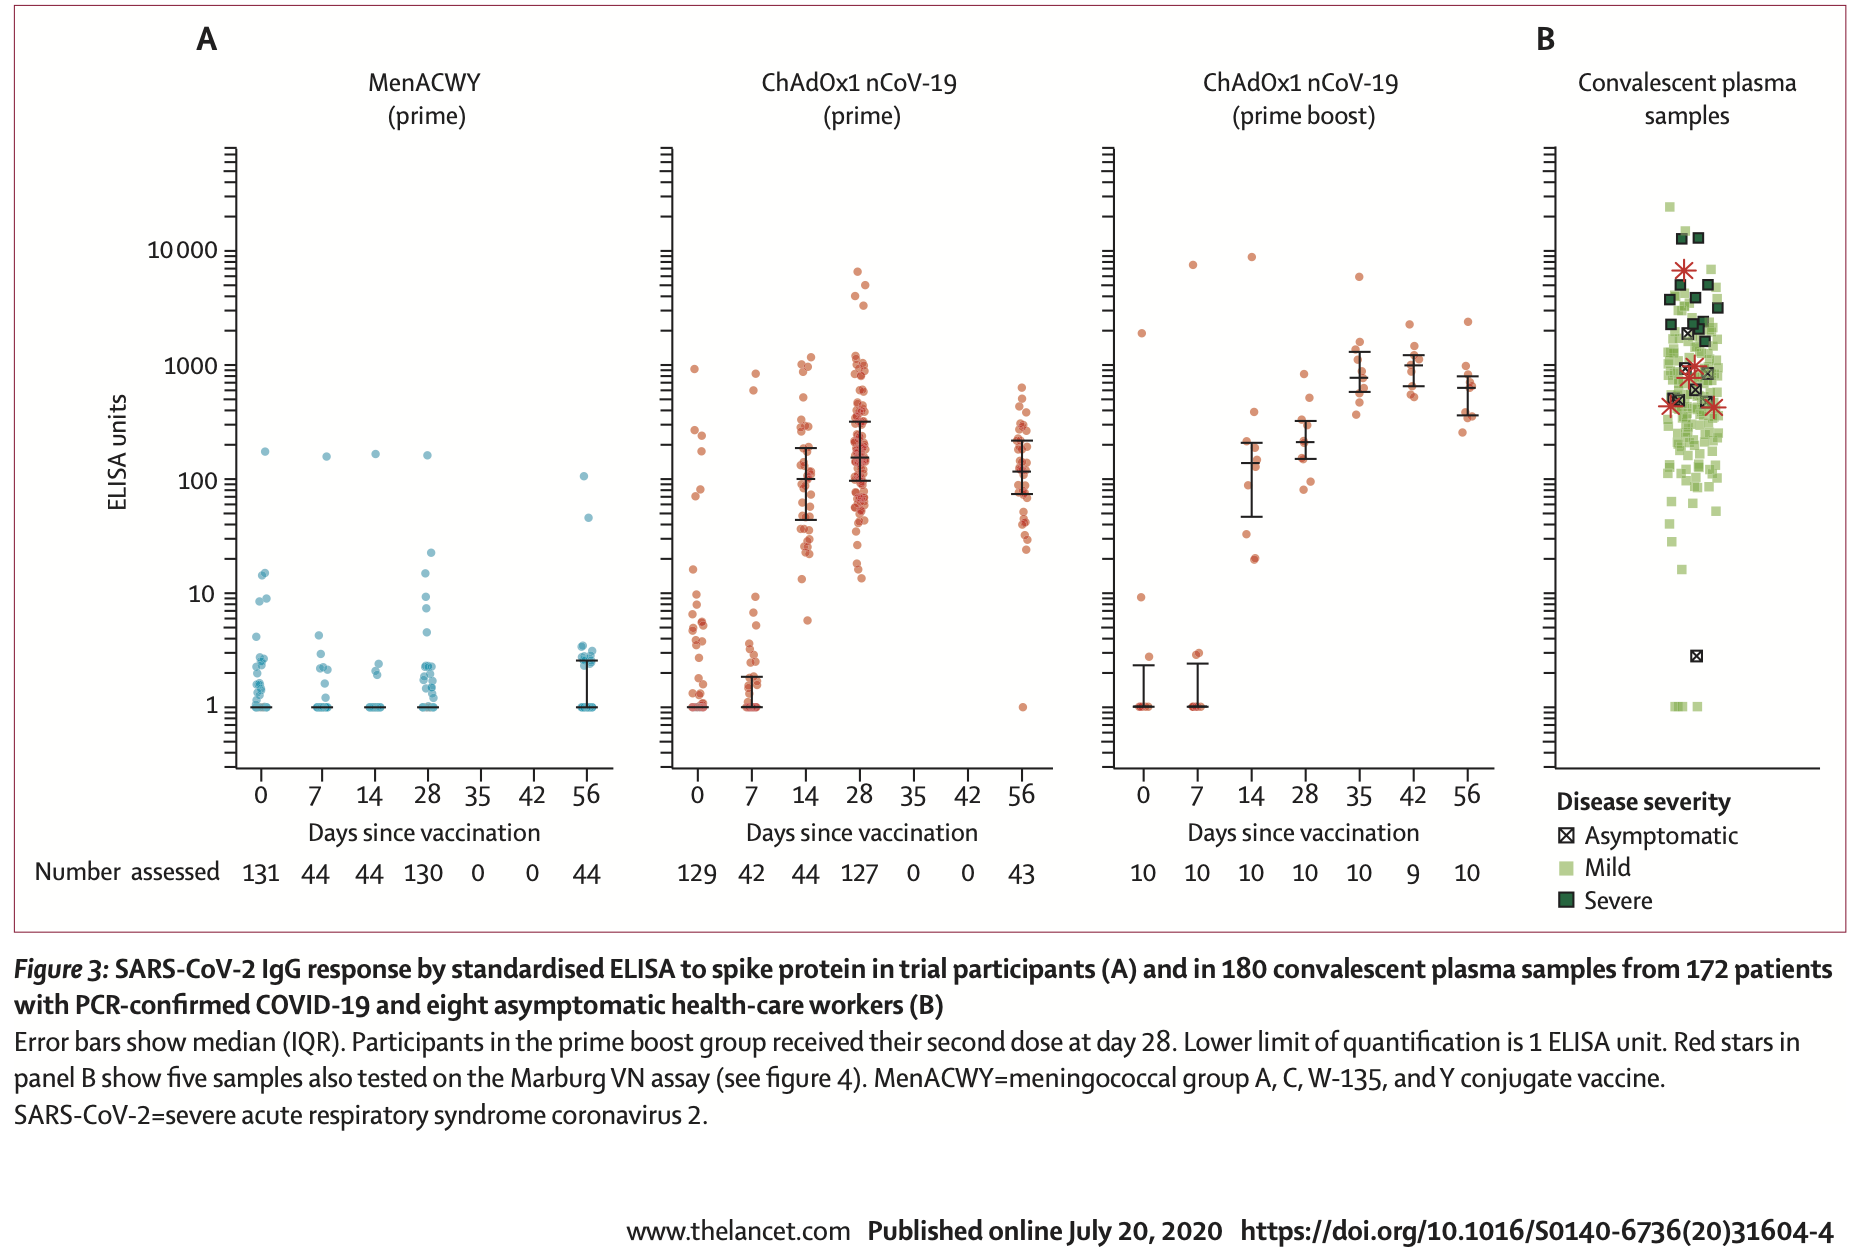
\includegraphics[width=0.75\linewidth]{downloadFigs4latex_002-motivating-examples/named-chunk} 

}



\end{knitrout}

	\vspace*{0.4cm}


\begin{enumerate}
	\item What levels of immunity are found in patients who have recovered from  COVID-19? (panel B) 
	\item Relative to these what levels of immunity are found in persons who have received the ChAdOx1 nCoV-19 vaccine? Compare panel A (prime, 28 days) vs panel B.   
\end{enumerate}

	
\end{frame}



\begin{frame}[fragile]{What levels of immunity are found in patients who have recovered from  COVID-19?\footnote{\tiny{Data were (imperfectly) scraped from the Postscript file ``behind'' the pdf file by Dr. Hanley}} }

	
\begin{knitrout}\tiny
\definecolor{shadecolor}{rgb}{0.969, 0.969, 0.969}\color{fgcolor}\begin{kframe}
\begin{alltt}
\hlstd{path} \hlkwb{<-}
  \hlstr{"http://www.biostat.mcgill.ca/hanley/statbook/immunogenicityChAdOx1.nCoV-19vaccine.txt"}
\hlstd{ds} \hlkwb{<-} \hlkwd{read.table}\hlstd{(path)}
\hlkwd{head}\hlstd{(ds)}
\end{alltt}
\begin{verbatim}
##   RefIndexCategory IgGResponse.log10.ElisaUnits
## 1     Convalescent                         2.56
## 2     Convalescent                         2.74
## 3     Convalescent                         2.79
## 4     Convalescent                         3.32
## 5     Convalescent                         3.15
## 6     Convalescent                         2.35
\end{verbatim}
\begin{alltt}
\hlkwd{str}\hlstd{(ds)}
\end{alltt}
\begin{verbatim}
## 'data.frame':	307 obs. of  2 variables:
##  $ RefIndexCategory            : Factor w/ 2 levels "Convalescent",..: 1 1 1 1 1 1 1 1 1 1 ...
##  $ IgGResponse.log10.ElisaUnits: num  2.56 2.74 2.79 3.32 3.15 2.35 2.72 2.95 2.42 2.64 ...
\end{verbatim}
\begin{alltt}
\hlkwd{levels}\hlstd{(ds}\hlopt{$}\hlstd{RefIndexCategory)}
\end{alltt}
\begin{verbatim}
## [1] "Convalescent"             "Day28PostChAdOx1 nCoV-19"
\end{verbatim}
\end{kframe}
\end{knitrout}

\end{frame}



\begin{frame}[fragile]{What levels of immunity are found in patients who have recovered from  COVID-19?}


\begin{knitrout}\tiny
\definecolor{shadecolor}{rgb}{0.969, 0.969, 0.969}\color{fgcolor}\begin{kframe}
\begin{alltt}
\hlstd{natural} \hlkwb{<-} \hlstd{ds[ds}\hlopt{$}\hlstd{RefIndexCategory}\hlopt{==}\hlstr{"Convalescent"}\hlstd{,]}
\hlkwd{hist}\hlstd{(natural}\hlopt{$}\hlstd{IgGResponse.log10.ElisaUnits,}
     \hlkwc{breaks} \hlstd{=} \hlnum{20}\hlstd{,} \hlkwc{col} \hlstd{=} \hlstr{"lightblue"}\hlstd{)}
\end{alltt}
\end{kframe}

{\centering 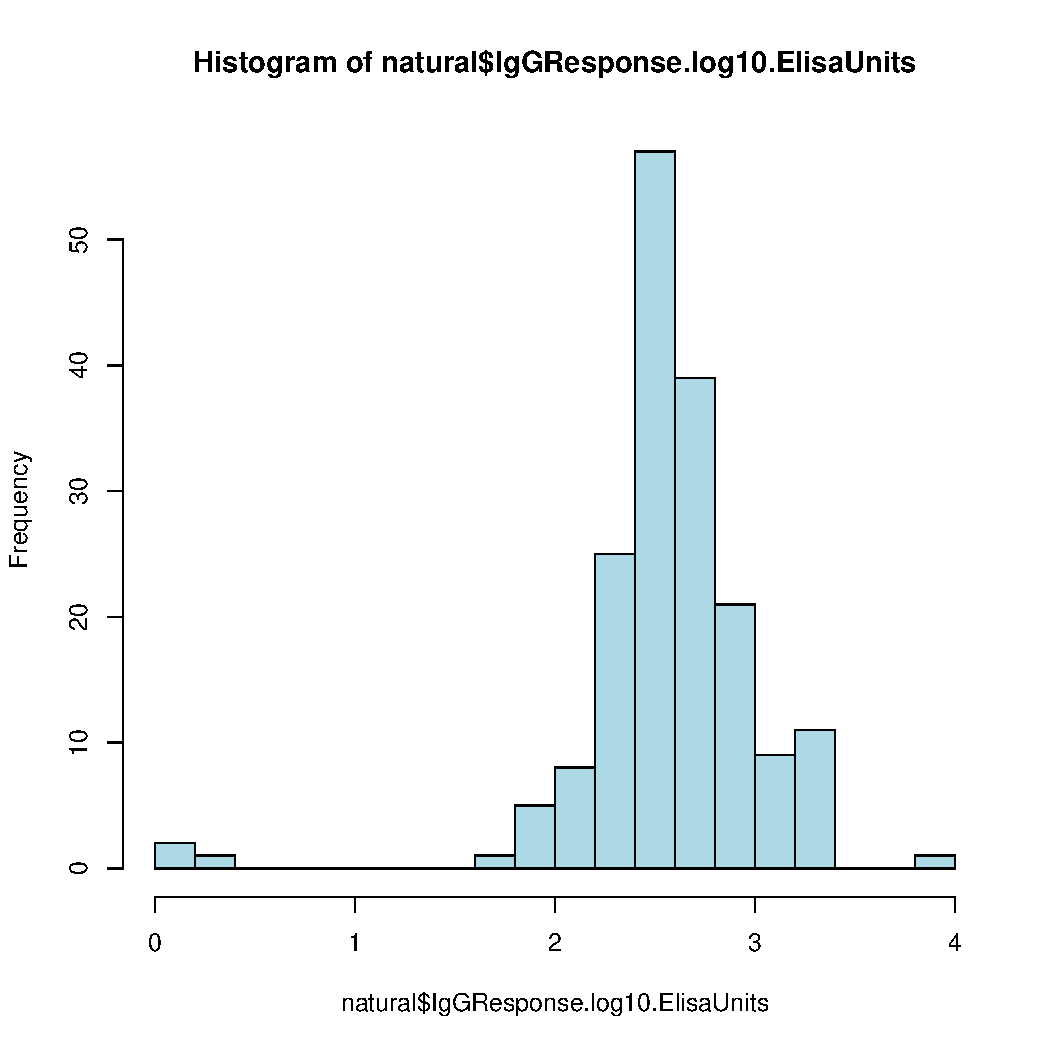
\includegraphics[width=0.6\linewidth]{figure/unnamed-chunk-1-1} 

}



\end{knitrout}

\end{frame}


\begin{frame}[fragile]{Three different methods of calculating the mean}

\begin{figure}
\begin{minipage}[h]{0.40\linewidth}
\begin{knitrout}\tiny
\definecolor{shadecolor}{rgb}{0.969, 0.969, 0.969}\color{fgcolor}\begin{kframe}
\begin{alltt}
\hlkwd{summary}\hlstd{(natural}\hlopt{$}\hlstd{IgGResponse.log10.ElisaUnits)}
\end{alltt}
\begin{verbatim}
##    Min. 1st Qu.  Median    Mean 3rd Qu.    Max. 
##   0.000   2.417   2.570   2.577   2.780   3.860
\end{verbatim}
\begin{alltt}
\hlkwd{boxplot}\hlstd{(natural}\hlopt{$}\hlstd{IgGResponse.log10.ElisaUnits,}
        \hlkwc{col} \hlstd{=} \hlstr{"lightblue"}\hlstd{,}
        \hlkwc{ylab} \hlstd{=} \hlstr{"Immunoglobulin G (IgG) response"}\hlstd{)}
\hlkwd{grid}\hlstd{(}\hlkwc{lty} \hlstd{=} \hlstr{"dashed"}\hlstd{)}
\end{alltt}
\end{kframe}

{\centering 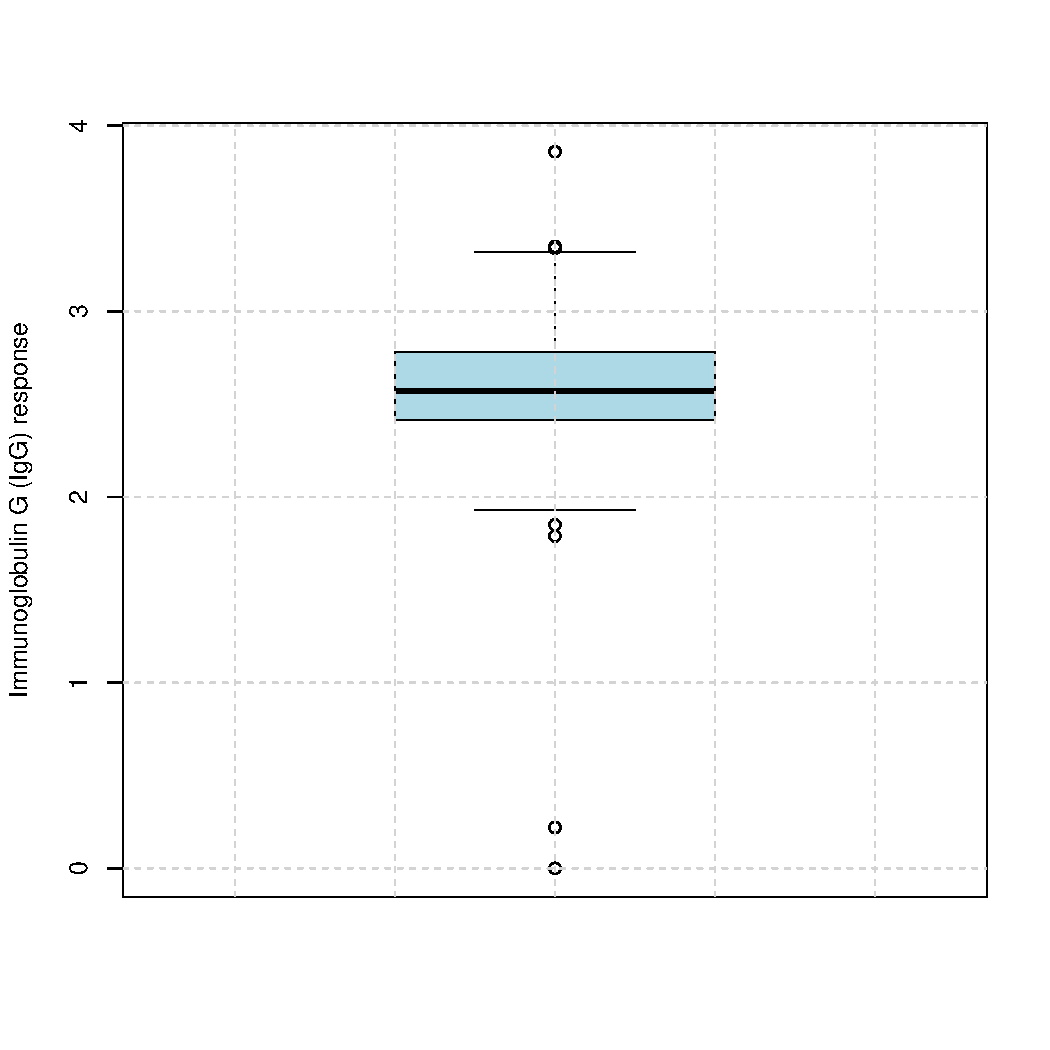
\includegraphics[width=0.99\linewidth]{figure/unnamed-chunk-2-1} 

}



\end{knitrout}

\end{minipage}
\hspace{0.4cm}
\begin{minipage}[h]{0.50\linewidth}
\begin{knitrout}\tiny
\definecolor{shadecolor}{rgb}{0.969, 0.969, 0.969}\color{fgcolor}\begin{kframe}
\begin{alltt}
\hlkwd{t.test}\hlstd{(natural}\hlopt{$}\hlstd{IgGResponse.log10.ElisaUnits)}
\end{alltt}
\begin{verbatim}
## One Sample t-test with natural$IgGResponse.log10.ElisaUnits 
## t = 75.0898, df = 179, p-value < 2.2e-16
## alternative hypothesis: true mean is not equal to 0 
## 95 percent confidence interval:
##  2.509603 2.645064 
## sample estimates:
## mean of x 
##  2.577333
\end{verbatim}
\begin{alltt}
\hlstd{fit1} \hlkwb{<-} \hlkwd{glm}\hlstd{(IgGResponse.log10.ElisaUnits} \hlopt{~} \hlnum{1}\hlstd{,} \hlkwc{data} \hlstd{= natural)}
\hlkwd{summary}\hlstd{(fit1)}
\end{alltt}
\begin{verbatim}
## 
## Coefficients:
##             Estimate Std. Error t value Pr(>|t|)    
## (Intercept)  2.57733    0.03432   75.09   <2e-16 ***
## ---
## Signif. codes:  0 '***' 0.001 '**' 0.01 '*' 0.05 '.' 0.1 ' ' 1
## 
## (Dispersion parameter for gaussian family taken to be 0.2120565)
## 
##     Null deviance: 37.958  on 179  degrees of freedom
## Residual deviance: 37.958  on 179  degrees of freedom
## AIC: 234.65
## 
## Number of Fisher Scoring iterations: 2
\end{verbatim}
\begin{alltt}
\hlkwd{confint}\hlstd{(fit1)}
\end{alltt}
\begin{verbatim}
##    2.5 %   97.5 % 
## 2.510061 2.644606
\end{verbatim}
\end{kframe}
\end{knitrout}
\end{minipage}
\end{figure}


\end{frame}



\begin{frame}[fragile]{Naturally vs. vaccine-induced response levels}
	
	
\begin{knitrout}\tiny
\definecolor{shadecolor}{rgb}{0.969, 0.969, 0.969}\color{fgcolor}\begin{kframe}
\begin{alltt}
\hlstd{p1} \hlkwb{<-} \hlkwd{ggplot}\hlstd{(}\hlkwc{data} \hlstd{= ds,} \hlkwc{mapping} \hlstd{=} \hlkwd{aes}\hlstd{(}\hlkwc{x} \hlstd{= RefIndexCategory,} \hlkwc{y} \hlstd{= IgGResponse.log10.ElisaUnits,}
    \hlkwc{fill} \hlstd{= RefIndexCategory))} \hlopt{+} \hlkwd{geom_jitter}\hlstd{(}\hlkwc{alpha} \hlstd{=} \hlnum{0.3}\hlstd{)} \hlopt{+} \hlkwd{theme_minimal}\hlstd{()} \hlopt{+} \hlkwd{theme}\hlstd{(}\hlkwc{legend.position} \hlstd{=} \hlstr{"none"}\hlstd{)}
\hlstd{p1} \hlopt{+} \hlkwd{geom_violin}\hlstd{()}
\hlstd{p1} \hlopt{+} \hlkwd{geom_boxplot}\hlstd{()}
\end{alltt}
\end{kframe}\begin{figure}

{\centering \subfloat[Violin plot\label{fig:unnamed-chunk-4-1}]{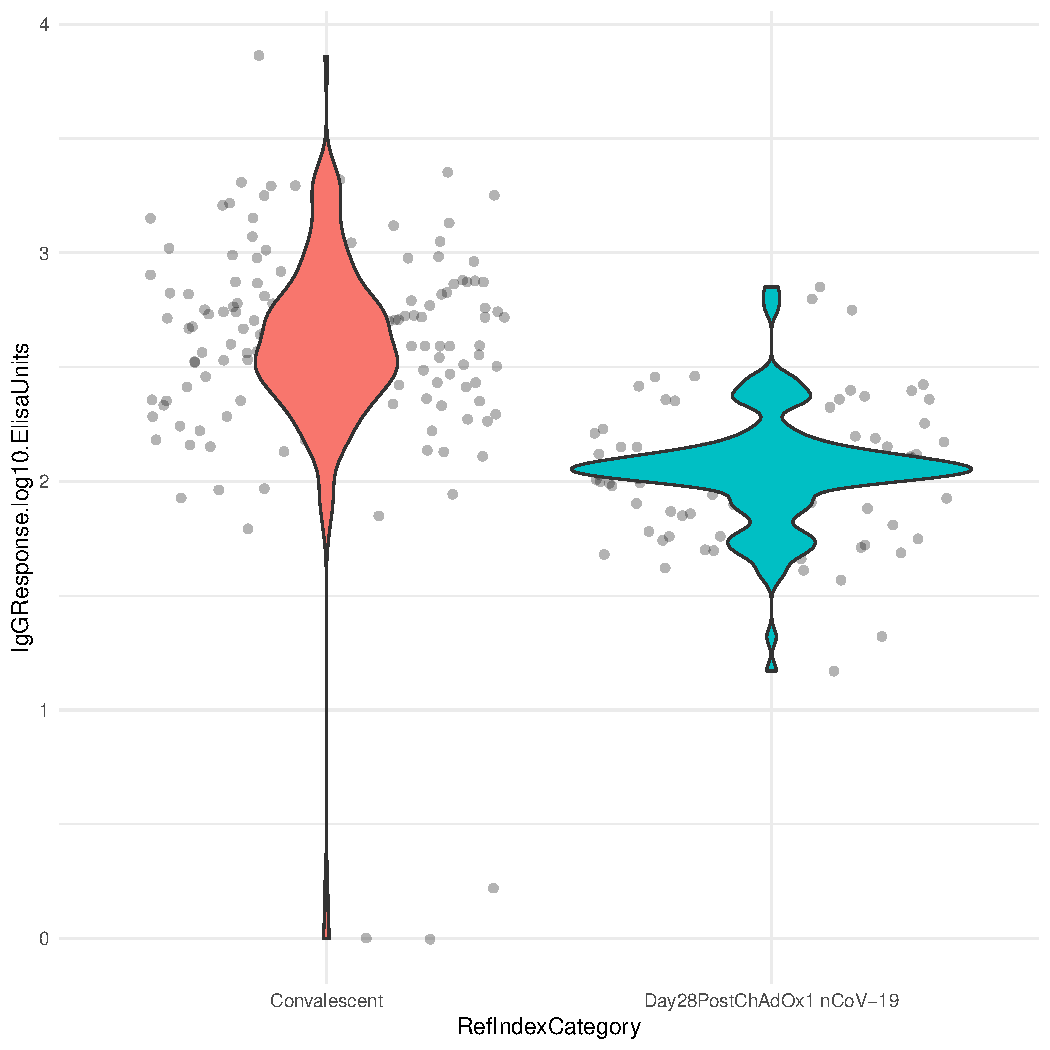
\includegraphics[width=0.5\linewidth]{figure/unnamed-chunk-4-1} }
\subfloat[Boxplot\label{fig:unnamed-chunk-4-2}]{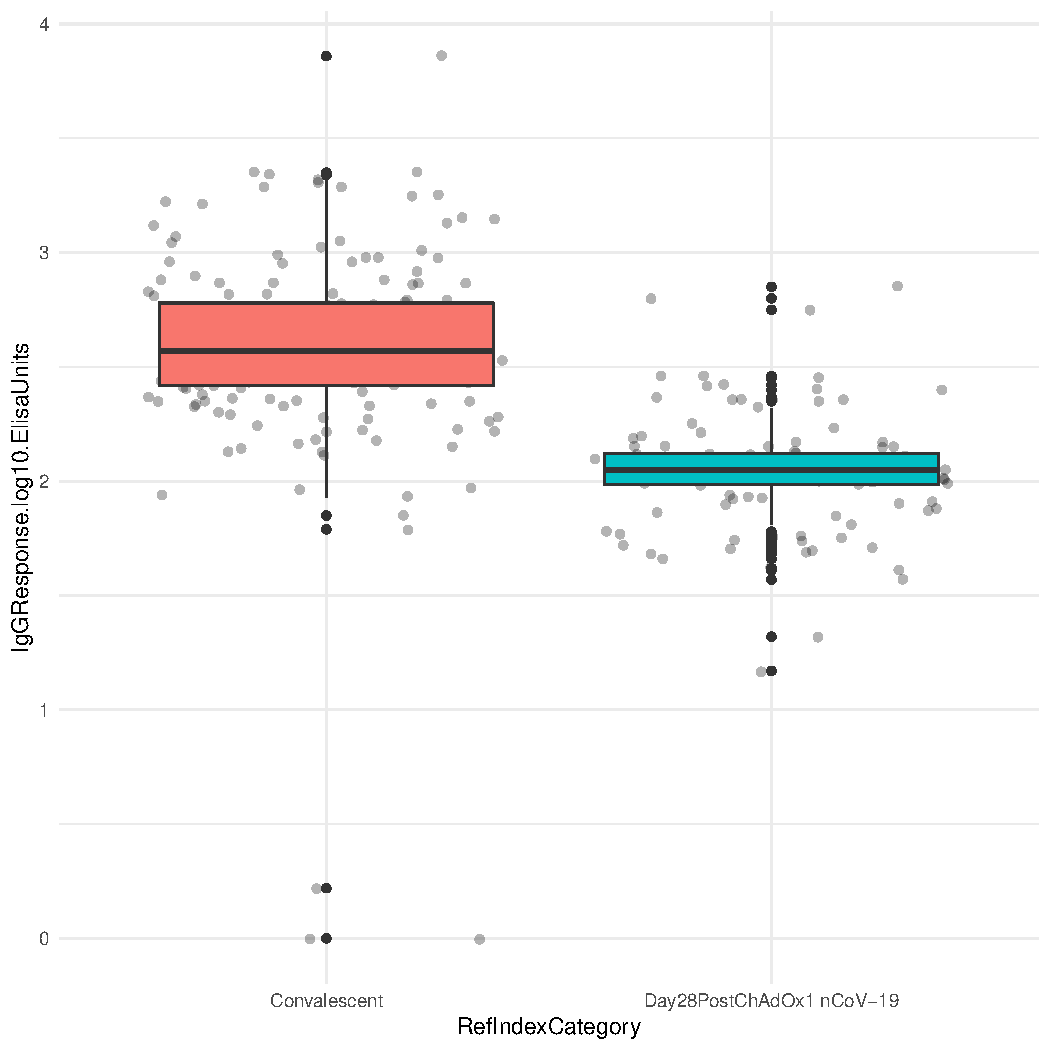
\includegraphics[width=0.5\linewidth]{figure/unnamed-chunk-4-2} }

}

\end{figure}


\end{knitrout}
	
\end{frame}



\begin{frame}[fragile]{Comparing means using classic methods}

\textbf{1. Numerical summary} \\

\begin{knitrout}\tiny
\definecolor{shadecolor}{rgb}{0.969, 0.969, 0.969}\color{fgcolor}\begin{kframe}
\begin{alltt}
\hlkwd{by}\hlstd{(ds}\hlopt{$}\hlstd{IgGResponse.log10.ElisaUnits,ds}\hlopt{$}\hlstd{RefIndexCategory,summary)}
\end{alltt}
\begin{verbatim}
## ds$RefIndexCategory: Convalescent
##    Min. 1st Qu.  Median    Mean 3rd Qu.    Max. 
##   0.000   2.417   2.570   2.577   2.780   3.860 
## ------------------------------------------------------------ 
## ds$RefIndexCategory: Day28PostChAdOx1 nCoV-19
##    Min. 1st Qu.  Median    Mean 3rd Qu.    Max. 
##   1.170   1.985   2.050   2.047   2.120   2.850
\end{verbatim}
\end{kframe}
\end{knitrout}
\pause

\vspace*{0.3in}

\textbf{2. Another ``dot'' test} \\

\begin{knitrout}\tiny
\definecolor{shadecolor}{rgb}{0.969, 0.969, 0.969}\color{fgcolor}\begin{kframe}
\begin{alltt}
\hlkwd{t.test}\hlstd{(IgGResponse.log10.ElisaUnits} \hlopt{~} \hlstd{RefIndexCategory,} \hlkwc{data} \hlstd{= ds)}
\end{alltt}
\begin{verbatim}
## Welch Two Sample t-test with IgGResponse.log10.ElisaUnits by RefIndexCategory 
## t = 13.1047, df = 284.781, p-value < 2.2e-16
## alternative hypothesis: true difference in means is not equal to 0 
## 95 percent confidence interval:
##  0.4510720 0.6105238 
## sample estimates:
##             mean in group Convalescent mean in group Day28PostChAdOx1 nCoV-19 
##                               2.577333                               2.046535
\end{verbatim}
\end{kframe}
\end{knitrout}

\end{frame}



\begin{frame}[fragile]{Comparing means using regression}
	
\textbf{3. Regression} \\
	
\begin{knitrout}\tiny
\definecolor{shadecolor}{rgb}{0.969, 0.969, 0.969}\color{fgcolor}\begin{kframe}
\begin{alltt}
\hlstd{fit2} \hlkwb{<-} \hlkwd{glm}\hlstd{(IgGResponse.log10.ElisaUnits} \hlopt{~} \hlstd{RefIndexCategory,} \hlkwc{data} \hlstd{= ds)}
\hlkwd{print}\hlstd{(}\hlkwd{summary}\hlstd{(fit2),} \hlkwc{signif.star} \hlstd{=} \hlnum{FALSE}\hlstd{)}
\end{alltt}
\begin{verbatim}
## 
## Coefficients:
##                                          Estimate Std. Error t value Pr(>|t|)
## (Intercept)                               2.57733    0.02874   89.67   <2e-16
## RefIndexCategoryDay28PostChAdOx1 nCoV-19 -0.53080    0.04469  -11.88   <2e-16
## 
## (Dispersion parameter for gaussian family taken to be 0.1487187)
## 
##     Null deviance: 66.339  on 306  degrees of freedom
## Residual deviance: 45.359  on 305  degrees of freedom
## AIC: 290.17
## 
## Number of Fisher Scoring iterations: 2
\end{verbatim}
\begin{alltt}
\hlkwd{confint}\hlstd{(fit2)}
\end{alltt}
\begin{verbatim}
##                                               2.5 %     97.5 %
## (Intercept)                               2.5209962  2.6336704
## RefIndexCategoryDay28PostChAdOx1 nCoV-19 -0.6183894 -0.4432064
\end{verbatim}
\end{kframe}
\end{knitrout}

\end{frame}


\begin{frame}[fragile]{Fitted regression line}
	
\begin{knitrout}\tiny
\definecolor{shadecolor}{rgb}{0.969, 0.969, 0.969}\color{fgcolor}\begin{kframe}
\begin{alltt}
\hlkwd{plot}\hlstd{(ds}\hlopt{$}\hlstd{RefIndexCategory, ds}\hlopt{$}\hlstd{IgGResponse.log10.ElisaUnits,} \hlkwc{pch}\hlstd{=}\hlnum{19}\hlstd{,} \hlkwc{cex}\hlstd{=}\hlnum{0.5}\hlstd{)}
\hlkwd{abline}\hlstd{(}\hlkwc{h} \hlstd{=} \hlkwd{seq}\hlstd{(}\hlnum{0}\hlstd{,}\hlnum{4}\hlstd{,}\hlnum{0.5}\hlstd{),}\hlkwc{col} \hlstd{=} \hlstr{"lightblue"}\hlstd{)}
\hlkwd{lines}\hlstd{(ds}\hlopt{$}\hlstd{RefIndexCategory, fit2}\hlopt{$}\hlstd{fitted.values,} \hlkwc{col} \hlstd{=} \hlstr{"red"}\hlstd{,} \hlkwc{lwd} \hlstd{=} \hlnum{3}\hlstd{)}
\end{alltt}
\end{kframe}\begin{figure}

{\centering 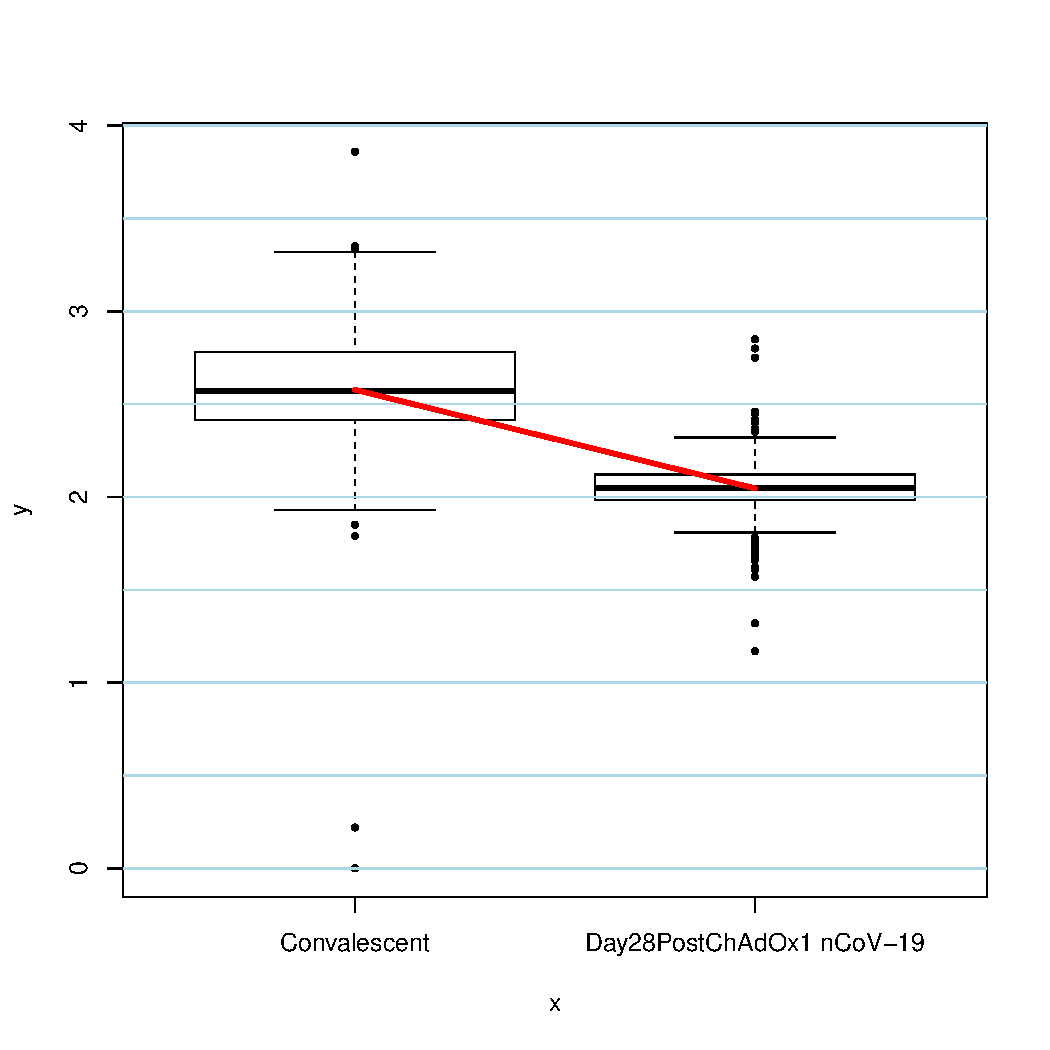
\includegraphics[width=0.5\linewidth]{figure/unnamed-chunk-8-1} 

}

\caption[The red line is the fitted regression from the previous slide]{The red line is the fitted regression from the previous slide.}\label{fig:unnamed-chunk-8}
\end{figure}


\end{knitrout}
	
\end{frame}




\section{Case study 2: Comparison of Estimated Rates of Coronavirus Disease 2019 (COVID-19) in Border Counties in Iowa Without a Stay-at-Home Order and Border Counties in Illinois With a Stay-at-Home Order}

\begin{frame}{Comparing Iowa and Illinois Cases\footnote{\tiny\url{https://jamanetwork.com/journals/jamanetworkopen/fullarticle/2766229}}}
	\centering
	
\includegraphics[scale=0.25]{002-masks.png}	
\end{frame}


\begin{frame}[fragile]{Are the difference in curves real? Or just random variation?}

\begin{itemize}
	\item This study compared COVID-19 cases in border counties in \textcolor{red}{Iowa, which did not issue a stay-at-home order}, with cases in border counties in \textcolor{blue}{Illinois, which did issue a stay-at-home order}.
\end{itemize}

\begin{knitrout}\tiny
\definecolor{shadecolor}{rgb}{0.969, 0.969, 0.969}\color{fgcolor}

{\centering 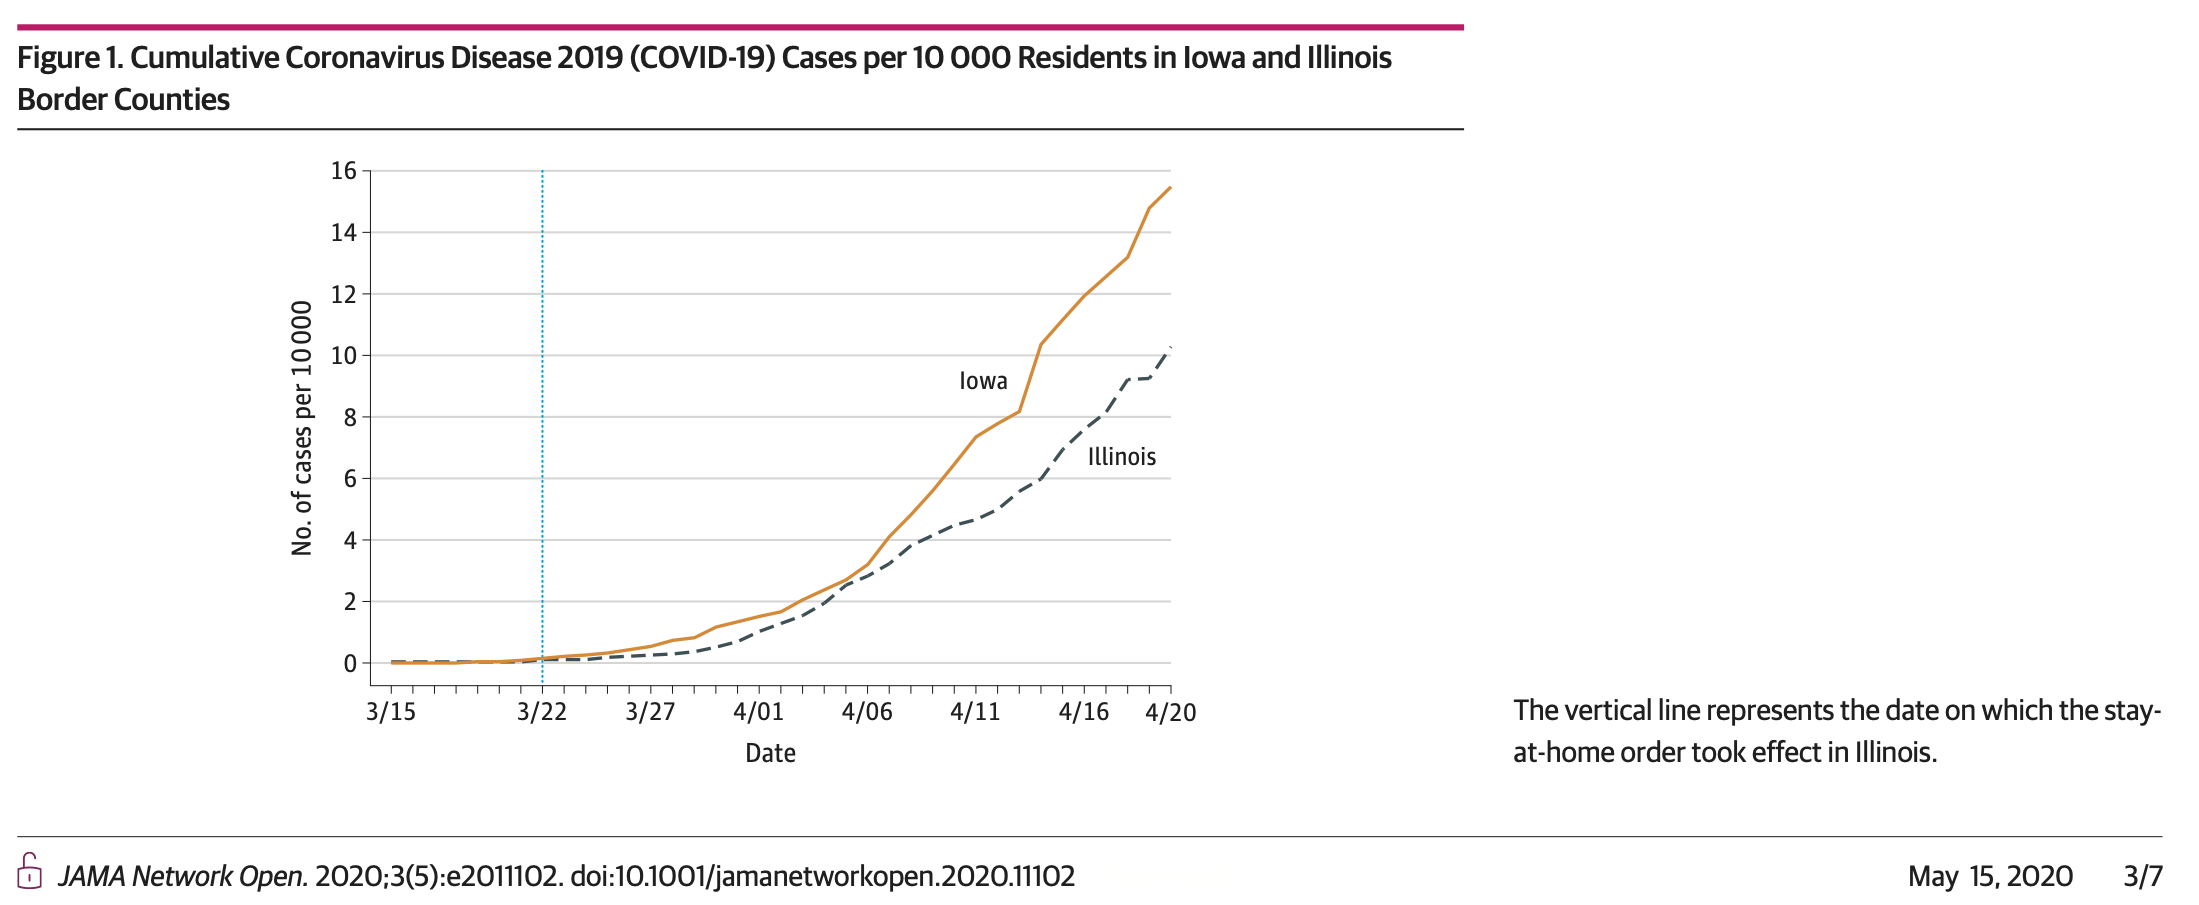
\includegraphics[width=1\linewidth]{downloadFigs4latex_002-motivating-examples/masks} 

}



\end{knitrout}

\end{frame}





\begin{frame}[fragile]{Freely available county level data from NYTimes\footnote{\tiny{\url{https://github.com/nytimes/covid-19-data}}}}
	
\begin{knitrout}\tiny
\definecolor{shadecolor}{rgb}{0.969, 0.969, 0.969}\color{fgcolor}\begin{kframe}
\begin{alltt}
\hlkwd{library}\hlstd{(covdata)} \hlcom{# remotes::install_github("kjhealy/covdata")}
\hlkwd{library}\hlstd{(dplyr);} \hlkwd{library}\hlstd{(tidyr);} \hlkwd{library}\hlstd{(ggplot2);} \hlkwd{library}\hlstd{(readr)}

\hlcom{# get population data from https://covid19.census.gov/datasets/}
\hlstd{pop_county} \hlkwb{<-} \hlkwd{read_csv}\hlstd{(}\hlstr{"https://opendata.arcgis.com/datasets/21843f238cbb46b08615fc53e19e0daf_1.csv"}\hlstd{)} \hlopt
              \hlstd{dplyr}\hlopt{::}\hlkwd{rename}\hlstd{(}\hlkwc{fips} \hlstd{= GEOID,} \hlkwc{population} \hlstd{= B01001_001E,} \hlkwc{state} \hlstd{= State)} \hlopt
              \hlstd{dplyr}\hlopt{::}\hlkwd{select}\hlstd{(state, fips, population)}

\hlstd{county_level} \hlkwb{<-} \hlstd{nytcovcounty} \hlopt
                \hlstd{dplyr}\hlopt{::}\hlkwd{left_join}\hlstd{(pop_county,} \hlkwc{by} \hlstd{=} \hlkwd{c}\hlstd{(}\hlstr{"state"}\hlstd{,}\hlstr{"fips"}\hlstd{))} \hlopt
                \hlstd{dplyr}\hlopt{::}\hlkwd{mutate}\hlstd{(}\hlkwc{cases.per.10k} \hlstd{= cases}\hlopt{/}\hlstd{population} \hlopt{*} \hlnum{1e4}\hlstd{)} \hlopt
                \hlstd{dplyr}\hlopt{::}\hlkwd{filter}\hlstd{(state} \hlopt \hlkwd{c}\hlstd{(}\hlstr{"Iowa"}\hlstd{,}\hlstr{"Illinois"}\hlstd{))} \hlopt
                \hlstd{dplyr}\hlopt{::}\hlkwd{group_by}\hlstd{(county)}

\hlstd{pop_state} \hlkwb{<-} \hlstd{pop_county} \hlopt
             \hlstd{dplyr}\hlopt{::}\hlkwd{group_by}\hlstd{(state)} \hlopt
             \hlstd{dplyr}\hlopt{::}\hlkwd{summarise}\hlstd{(}\hlkwc{population} \hlstd{=} \hlkwd{sum}\hlstd{(population,} \hlkwc{na.rm} \hlstd{=} \hlnum{TRUE}\hlstd{))}

\hlstd{state_level} \hlkwb{<-} \hlstd{county_level} \hlopt
               \hlstd{dplyr}\hlopt{::}\hlkwd{group_by}\hlstd{(state, date)} \hlopt
               \hlstd{dplyr}\hlopt{::}\hlkwd{filter}\hlstd{(date} \hlopt{>=} \hlstr{"2020-03-15"}\hlstd{)} \hlopt
               \hlstd{dplyr}\hlopt{::}\hlkwd{summarise}\hlstd{(}\hlkwc{cases} \hlstd{=} \hlkwd{sum}\hlstd{(cases))} \hlopt
               \hlstd{dplyr}\hlopt{::}\hlkwd{left_join}\hlstd{(pop_state,} \hlkwc{by} \hlstd{=} \hlstr{"state"}\hlstd{)} \hlopt
               \hlstd{dplyr}\hlopt{::}\hlkwd{mutate}\hlstd{(}\hlkwc{cases.per.10k} \hlstd{= cases} \hlopt{/} \hlstd{population} \hlopt{*} \hlnum{1e4}\hlstd{,} \hlkwc{state} \hlstd{=} \hlkwd{factor}\hlstd{(state),}
                             \hlkwc{time} \hlstd{=} \hlkwd{as.numeric}\hlstd{(date} \hlopt{-} \hlkwd{min}\hlstd{(date))} \hlopt{+} \hlnum{1}\hlstd{)}
\hlkwd{head}\hlstd{(state_level)}
\end{alltt}
\begin{verbatim}
## # A tibble: 6 x 6
## # Groups:   state [1]
##   state    date       cases population cases.per.10k  time
##   <fct>    <date>     <dbl>      <dbl>         <dbl> <dbl>
## 1 Illinois 2020-03-15    94   12821497        0.0733     1
## 2 Illinois 2020-03-16   104   12821497        0.0811     2
## 3 Illinois 2020-03-17   159   12821497        0.124      3
## 4 Illinois 2020-03-18   286   12821497        0.223      4
## 5 Illinois 2020-03-19   420   12821497        0.328      5
## 6 Illinois 2020-03-20   583   12821497        0.455      6
\end{verbatim}
\end{kframe}
\end{knitrout}
	
\end{frame}



\begin{frame}[fragile]{County level cases for Iowa and Illinois - log10 scale}
	
\begin{knitrout}\tiny
\definecolor{shadecolor}{rgb}{0.969, 0.969, 0.969}\color{fgcolor}\begin{kframe}
\begin{alltt}
\hlkwd{ggplot}\hlstd{(}\hlkwc{data} \hlstd{= county_level,} \hlkwc{mapping} \hlstd{=} \hlkwd{aes}\hlstd{(}\hlkwc{x} \hlstd{= date,} \hlkwc{y} \hlstd{= cases,} \hlkwc{group} \hlstd{= county))} \hlopt{+}
  \hlkwd{geom_line}\hlstd{(}\hlkwc{size} \hlstd{=} \hlnum{0.25}\hlstd{,} \hlkwc{color} \hlstd{=} \hlstr{"gray20"}\hlstd{)} \hlopt{+}
  \hlkwd{scale_x_date}\hlstd{(}\hlkwc{date_breaks} \hlstd{=} \hlstr{"1 month"}\hlstd{,} \hlkwc{date_labels} \hlstd{=} \hlstr{"%b"}\hlstd{)}\hlopt{+}
  \hlkwd{scale_y_log10}\hlstd{(}\hlkwc{labels} \hlstd{= scales}\hlopt{::}\hlkwd{label_number_si}\hlstd{())} \hlopt{+}
  \hlkwd{guides}\hlstd{(}\hlkwc{color} \hlstd{=} \hlnum{FALSE}\hlstd{)} \hlopt{+} \hlkwd{facet_wrap}\hlstd{(}\hlopt{~} \hlstd{state,} \hlkwc{ncol} \hlstd{=} \hlnum{2}\hlstd{)} \hlopt{+}
  \hlkwd{labs}\hlstd{(}\hlkwc{title} \hlstd{=} \hlstr{"COVID-19 Cases in Iowa and Illinois by County"}\hlstd{,}
       \hlkwc{x} \hlstd{=} \hlstr{"Date"}\hlstd{,} \hlkwc{y} \hlstd{=} \hlstr{"No. of cases (log10 scale)"}\hlstd{,} \hlkwc{caption} \hlstd{=} \hlstr{"Data: The New York Times"}\hlstd{)} \hlopt{+}
  \hlkwd{theme_minimal}\hlstd{()}
\end{alltt}
\end{kframe}

{\centering 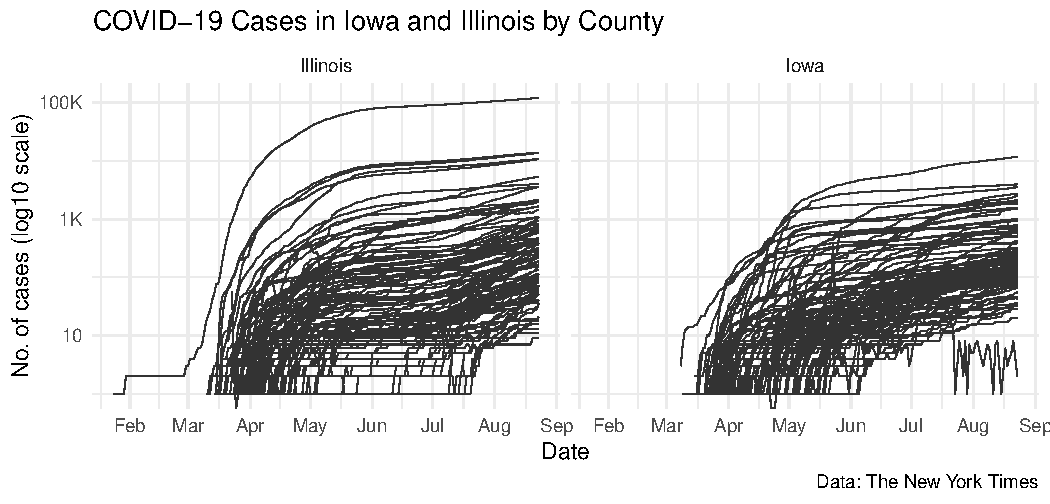
\includegraphics[width=\maxwidth]{figure/nytcases-1} 

}



\end{knitrout}
	
\end{frame}




\begin{frame}[fragile]{County level cases for Iowa and Illinois - per capita}
	
\begin{knitrout}\tiny
\definecolor{shadecolor}{rgb}{0.969, 0.969, 0.969}\color{fgcolor}\begin{kframe}
\begin{alltt}
\hlkwd{ggplot}\hlstd{(}\hlkwc{data} \hlstd{= county_level,} \hlkwc{mapping} \hlstd{=} \hlkwd{aes}\hlstd{(}\hlkwc{x} \hlstd{= date,} \hlkwc{y} \hlstd{= cases.per.10k,} \hlkwc{group} \hlstd{= county))} \hlopt{+}
  \hlkwd{geom_line}\hlstd{(}\hlkwc{size} \hlstd{=} \hlnum{0.25}\hlstd{,} \hlkwc{color} \hlstd{=} \hlstr{"gray20"}\hlstd{)} \hlopt{+}
  \hlkwd{scale_x_date}\hlstd{(}\hlkwc{date_breaks} \hlstd{=} \hlstr{"1 month"}\hlstd{,} \hlkwc{date_labels} \hlstd{=} \hlstr{"%b"}\hlstd{)}\hlopt{+}
  \hlkwd{scale_y_continuous}\hlstd{(}\hlkwc{labels} \hlstd{= scales}\hlopt{::}\hlkwd{label_number_si}\hlstd{())} \hlopt{+}
  \hlkwd{guides}\hlstd{(}\hlkwc{color} \hlstd{=} \hlnum{FALSE}\hlstd{)} \hlopt{+} \hlkwd{facet_wrap}\hlstd{(}\hlopt{~} \hlstd{state,} \hlkwc{ncol} \hlstd{=} \hlnum{2}\hlstd{)} \hlopt{+}
  \hlkwd{labs}\hlstd{(}\hlkwc{title} \hlstd{=} \hlstr{"COVID-19 Cases in Iowa and Illinois by County"}\hlstd{,}
       \hlkwc{x} \hlstd{=} \hlstr{"Date"}\hlstd{,} \hlkwc{y} \hlstd{=} \hlstr{"No. of cases per 10 000"}\hlstd{,} \hlkwc{caption} \hlstd{=} \hlstr{"Data: The New York Times"}\hlstd{)} \hlopt{+}
  \hlkwd{theme_minimal}\hlstd{()}
\end{alltt}
\end{kframe}

{\centering 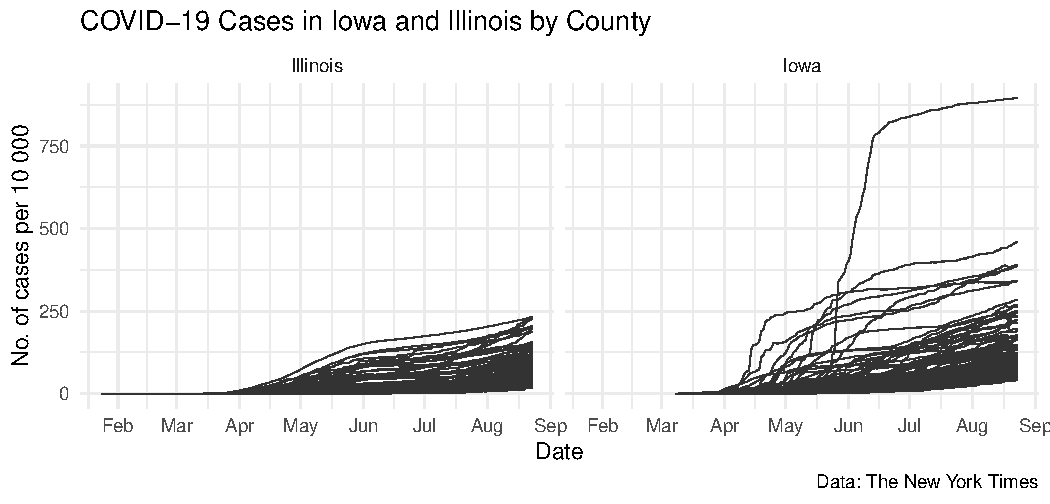
\includegraphics[width=\maxwidth]{figure/nytcapita-1} 

}



\end{knitrout}
	
\end{frame}



\begin{frame}[fragile]{State level cases for Iowa and Illinois - per capita}
	
\begin{knitrout}\tiny
\definecolor{shadecolor}{rgb}{0.969, 0.969, 0.969}\color{fgcolor}\begin{kframe}
\begin{alltt}
\hlkwd{ggplot}\hlstd{(}\hlkwc{data} \hlstd{= state_level,} \hlkwc{mapping} \hlstd{=} \hlkwd{aes}\hlstd{(}\hlkwc{x} \hlstd{= date,} \hlkwc{y} \hlstd{= cases.per.10k,} \hlkwc{color} \hlstd{= state))} \hlopt{+}
  \hlkwd{geom_line}\hlstd{(}\hlkwc{size} \hlstd{=} \hlnum{1}\hlstd{)} \hlopt{+}
  \hlkwd{scale_x_date}\hlstd{(}\hlkwc{date_breaks} \hlstd{=} \hlstr{"1 month"}\hlstd{,} \hlkwc{date_labels} \hlstd{=} \hlstr{"%b"}\hlstd{)}\hlopt{+}
  \hlkwd{scale_y_continuous}\hlstd{(}\hlkwc{labels} \hlstd{= scales}\hlopt{::}\hlkwd{label_number_si}\hlstd{())} \hlopt{+}
  \hlkwd{labs}\hlstd{(}\hlkwc{title} \hlstd{=} \hlstr{"COVID-19 Cases in Iowa and Illinois"}\hlstd{,}
       \hlkwc{subtitle} \hlstd{=} \hlstr{"Cases since March 15, 2020"}\hlstd{,}
       \hlkwc{x} \hlstd{=} \hlstr{"Date"}\hlstd{,} \hlkwc{y} \hlstd{=} \hlstr{"No. of cases per 10 000"}\hlstd{,} \hlkwc{caption} \hlstd{=} \hlstr{"Data: The New York Times"}\hlstd{)} \hlopt{+}
  \hlkwd{theme_minimal}\hlstd{()}
\end{alltt}
\end{kframe}

{\centering 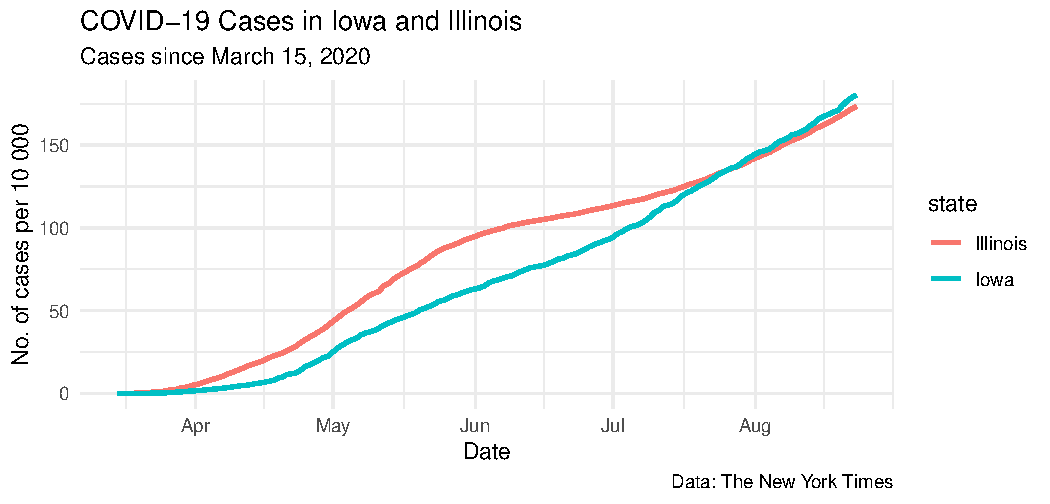
\includegraphics[width=\maxwidth]{figure/nytcapitastate-1} 

}



\end{knitrout}
	
\end{frame}


\begin{frame}[fragile]{Are the findings in the paper reproducible?}
	
\begin{knitrout}\tiny
\definecolor{shadecolor}{rgb}{0.969, 0.969, 0.969}\color{fgcolor}\begin{kframe}
\begin{alltt}
\hlstd{fit3} \hlkwb{<-} \hlkwd{glm}\hlstd{(cases.per.10k} \hlopt{~} \hlstd{state}\hlopt{*}\hlstd{time,} \hlkwc{data} \hlstd{= state_level)}
\hlkwd{summary}\hlstd{(fit3)}
\end{alltt}
\begin{verbatim}
## 
## Coefficients:
##                 Estimate Std. Error t value Pr(>|t|)    
## (Intercept)     -7.07540    1.22153  -5.792 1.66e-08 ***
## stateIowa      -17.88124    1.72751 -10.351  < 2e-16 ***
## time             1.10890    0.01300  85.300  < 2e-16 ***
## stateIowa:time   0.06078    0.01838   3.306  0.00105 ** 
## ---
## Signif. codes:  0 '***' 0.001 '**' 0.01 '*' 0.05 '.' 0.1 ' ' 1
## 
## (Dispersion parameter for gaussian family taken to be 59.87398)
## 
##     Null deviance: 953056  on 323  degrees of freedom
## Residual deviance:  19160  on 320  degrees of freedom
## AIC: 2251.3
## 
## Number of Fisher Scoring iterations: 2
\end{verbatim}
\end{kframe}
\end{knitrout}
	
\end{frame}


\begin{frame}[fragile]{Model-based predictions}
	
\begin{knitrout}\tiny
\definecolor{shadecolor}{rgb}{0.969, 0.969, 0.969}\color{fgcolor}\begin{kframe}
\begin{alltt}
\hlkwd{library}\hlstd{(ggeffects)}
\hlstd{ggeffects}\hlopt{::}\hlkwd{ggpredict}\hlstd{(fit3,} \hlkwc{terms} \hlstd{=} \hlstr{"state"}\hlstd{)} \hlopt
  \hlkwd{plot}\hlstd{()}
\end{alltt}
\end{kframe}

{\centering 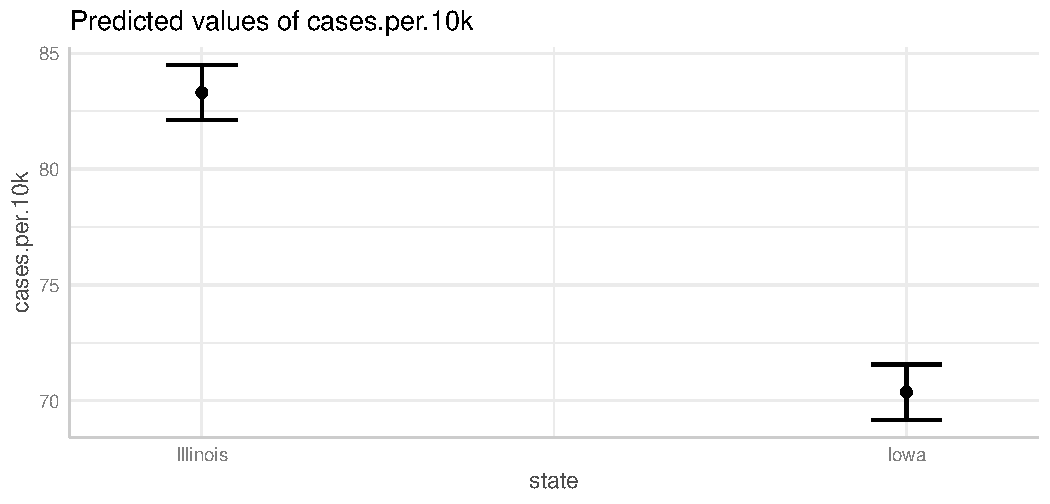
\includegraphics[width=\maxwidth]{figure/nytcapitastatemodel2-1} 

}



\end{knitrout}
	
\end{frame}


%\begin{frame}[allowframebreaks]
%\nocite{breiman1984classification}
%	\nocite{friedman2001elements}
%	\nocite{james2013introduction}
%	\nocite{lopez2015arbres}
%	\frametitle{References}
%\printbibliography
%\end{frame}


\begin{frame}[fragile]{Session Info}
	\tiny
	
\begin{knitrout}\tiny
\definecolor{shadecolor}{rgb}{0.969, 0.969, 0.969}\color{fgcolor}\begin{kframe}
\begin{verbatim}
R version 3.6.2 (2019-12-12)
Platform: x86_64-pc-linux-gnu (64-bit)
Running under: Pop!_OS 19.10

Matrix products: default
BLAS:   /usr/lib/x86_64-linux-gnu/openblas/libblas.so.3
LAPACK: /usr/lib/x86_64-linux-gnu/libopenblasp-r0.3.7.so

attached base packages:
[1] tools     stats     graphics  grDevices utils     datasets  methods  
[8] base     

other attached packages:
 [1] ggeffects_0.14.1   covdata_0.4.4      NCStats_0.4.7      FSA_0.8.30        
 [5] forcats_0.5.0      stringr_1.4.0      dplyr_1.0.2        purrr_0.3.4       
 [9] readr_1.3.1        tidyr_1.1.2        tibble_3.0.3       ggplot2_3.3.2.9000
[13] tidyverse_1.3.0    knitr_1.29        

loaded via a namespace (and not attached):
 [1] sjlabelled_1.1.3   tidyselect_1.1.0   xfun_0.16          haven_2.3.1       
 [5] snakecase_0.11.0   colorspace_1.4-1   vctrs_0.3.4        generics_0.0.2    
 [9] utf8_1.1.4         rlang_0.4.7        pillar_1.4.6       glue_1.4.2        
[13] withr_2.2.0        DBI_1.1.0          dbplyr_1.4.2       modelr_0.1.5      
[17] readxl_1.3.1       lifecycle_0.2.0    plyr_1.8.6         munsell_0.5.0     
[21] gtable_0.3.0       cellranger_1.1.0   rvest_0.3.5        evaluate_0.14     
[25] labeling_0.3       curl_4.3           fansi_0.4.1        highr_0.8         
[29] broom_0.7.0        Rcpp_1.0.4.6       scales_1.1.1       backports_1.1.9   
[33] formatR_1.7        jsonlite_1.7.0     farver_2.0.3       fs_1.3.2          
[37] TeachingDemos_2.12 digest_0.6.25      hms_0.5.3          stringi_1.4.6     
[41] insight_0.8.1      grid_3.6.2         cli_2.0.2          magrittr_1.5      
[45] crayon_1.3.4       pkgconfig_2.0.3    ellipsis_0.3.1     MASS_7.3-51.5     
[49] xml2_1.3.0         reprex_0.3.0       lubridate_1.7.4    assertthat_0.2.1  
[53] httr_1.4.1         rstudioapi_0.11    R6_2.4.1           compiler_3.6.2    
\end{verbatim}
\end{kframe}
\end{knitrout}
	
\end{frame}

\end{document}
